\pagestyle{plain}
\pagenumbering{arabic}
\setcounter{page}{1}
\chapter{\uppercase{Introduction}}
\section{Purpose}
The transport of photons and electrons has many applications. One of them is 
radiotherapy. Radiotherapy uses photons and charged particles to 
damage the DNA of cancerous cells. When using photons, free electrons are 
generated and ionize the environment to create free radicals that damage the cells. 
The absorbed dose, defined as the energy deposited per unit of mass, is used to 
gauge whether a cell will die due to the radiation or not. Several methods can be
applied to compute the dose distribution in the body: semi-analytic,
deterministic, and Monte-Carlo methods. Monte-Carlo methods yield very
accurate results, however they are slow to converge and remain too slow for
effective clinical use \cite{acuros,comet}. Semi-analytic methods, such as
pencil-beam convolution and convolution-superposition, employ pre-calculated
Monte-Carlo dose kernels, which are then locally scaled to approximate photon
and electron transport in the presence of heterogeneities. These methods
present some issues in the presence of large density gradients such as those
found at interfaces between different materials: air, bone, lung and soft
tissue \cite{acuros,seco,krieger}. The discrete ordinates ($S_n$) method has been 
shown to be quite accurate for electron and coupled electron-photon transport 
\cite{morel_81,accuracy_1,accuracy_2}.  

One difficulty of this approach arises from the transport of electrons. Charged 
particles interact through Coulomb interactions with the  background medium. 
Such interactions predominately result in extremely small changes 
in particle direction and energy. These interactions are well characterized by the
Fokker-Planck limit of the Boltzmann equation \cite{fp_limit,morel_96}. In this limit,
the directional and energy changes are decoupled with the former modeled by the
continuous scattering operator and the latter modeled by the continuous-slowing-down 
operator. The mean-free-path and the directional change per scattering interaction 
go to zero while the momentum transfer (also called the transport-corrected 
scattering cross section) remains fixed.

When the scattering is highly forward-peaked, solving the $S_n$ transport equation 
can be challenging due to the slow convergence of standard iterative
algorithm, such as Source Iteration (SI). To speed up iterative convergence,
acceleration schemes such as Diffusion Synthetic Acceleration (DSA) and P1
Synthetic Acceleration (P1SA) are generally used for neutron transport 
\cite{dsa_ref}. These methods use a diffusion equation or the P1 equations,
and therefore, only the zeroth or the zeroth plus the first flux moment can be
accelerated. When the zeroth flux moment alone is a accelerated, these
schemes are stable (in this discussion, we ignore the possible issues due to
the possible issues due to the spatial discretization) but they are very
inefficient if the scattering is highly anisotropic. If both the zeroth and
the first flux moments are accelerated, the spectral radius of the continuous
scheme (i.e., without spatial discretization) with anisotropic scattering is
given by \cite{multisweep}:
\begin{equation}
\rho_{ani} = \max\(\rho_{iso},\frac{\mu c}{1-\mu_c}\)
\end{equation}
where $\rho_{iso}(<1)$ is the spectral radius when the scattering is
isotropic, $\mu$ $(\in [0,1])$ is the average scattering cosine, and $c$ $(\in
[0,1])$ is the scattering ratio. We see that when $\mu c > 0.5$, the scheme is
unstable. Several modifications have been proposed \cite{multisweep,russe} to
stabilize this acceleration scheme. However, for electron transport, the
scattering anisotropy is very large and some others techniques have to be
used. The angular multigrid method \cite{multigrid_1d} has proven to be very
effective to solve the $S_n$ equations with highly forward-peaked scattering
for one-dimensional slab geometry. Unfortunately, the extension of the angular
multigrid method to multidimensional geometries is unstable
\cite{multigrid_2d}. Pautz et al. added a diffusive filter to the angular
multigrid corrections as a stabilizer within the standard preconditioned
Source Iteration. This stabilized angular multigrid method converges faster
than DSA alone but the spectral radius can become arbitrary close to one for
highly anisotropic and high scattering ratio medium. In
\cite{multigrid_1d,multigrid_2d}, the authors used the traditional Source
Iteration method as solver. However, the system of linear equations can be
also be tackled using non stationary Krylov solvers, such as GMRES. A code
solving the $S_n$ equations using SI with DSA can easily be modified to use a
preconditioned Krylov solvers. In \cite{ttg}, the authors summarize the
advantageous features of GMRES as follows: ``using DSA as preconditioner for
GMRES(m) removes the consistency requirement that plagues DSA-accelerated
source iteration in multidimensional problems.'' Driven by this statement, we
will use the multidimensional angular multigrid method as a preconditioner for
GMRES in solving highly forward peaked scattering problems. Our hope is
that GMRES will be able to stabilize the proposed scheme without the use of a
filter and that the new scheme will have convergence properties similar to the
one-dimensional scheme. At the coarsest level of the angular multigrid, a DSA 
scheme or a P1SA scheme has to be used. The scheme that we will use is an 
adaptation of the Modified Interior Penalty DSA (MIP) \cite{mip}. This scheme 
was developed for discontinuous finite elements on triangular cells and it is 
symmetric and definite positive (SPD). We will adapt MIP to Bilinear
Discontinuous Finite elements (BLD) on rectangular cells and to PieceWise Linear 
Discontinuous Finite elements (PWLD) \cite{pwld_2d,pwld_3d} on arbitrary
polygonal cells. Polygonal cells can potentially reduce the number of unknowns in 
our mesh, while maintaining symmetry within the mesh. We show this potential 
reduction in number of unknowns for a hexagonal cell versus the same space divided 
using triangles:
\begin{figure}[H]
\centering
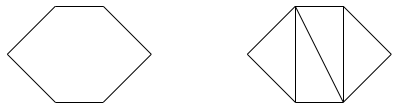
\includegraphics[width=0.5\textwidth]{./Introduction/hex_tri_cells}
\caption{Hexagonal cell versus triangle cells}
\end{figure}
We see that if there is one unknown per vertices, the hexagonal cell has 6
unknowns compared to the 12 unknowns of triangle cells. Polygonal cells can
also be used for adaptive mesh refinement (AMR) problems without having to
deal with hanging nodes \cite{arbitrary_hanging_nodes,dealII_hanging_nodes,
locally_hanging_nodes}. The left cell on the figure below is a pentagon whereas 
the two cells on the right are quadrilaterals:
\begin{figure}[H]
\centering

\includegraphics[width=0.3\textwidth]{./Introduction/amr}
\caption{AMR mesh}
\end{figure}
Using MIP requires us to solve SPD equations. This has usually been done using 
conjugate gradient preconditioned by SSOR, but in this research we will test the 
effectiveness of algebraic multigrid methods (AMG) to precondition the Krylov solver 
\cite{amg,amg_course}. Algebraic multigrid methods allow to use multigrid
techniques when there is no grid or that the mesh is unstructured. Instead of
using a succession of grids based on the geometry of the problems, the grids
are based on properties of the matrix. This allows to use AMG as black-box
solvers or preconditioners.

\section{Linear Boltzmann equation}
Charged particles transport can be described by the linear Boltzmann equation 
\cite{morel_81,galerkin_morel,cepxs}:
\begin{equation}
  \begin{split}
    & \bo\cdot \bn \psi(\br,\bo,E) + \Sigma_t(\br,E)\psi(\br,\bo,E) = 
    \int_0^{\infty}dE'\int_{4\pi}d\bo'\ \Sigma_s(\br,\bo'\cdot\bo,E'\rightarrow E)\\
    &\psi(\br,\bo',E')+Q(\br,\bo,E)
  \end{split}
\label{transport_p}
\end{equation}
where:
\begin{itemize}
\item $\bo = (\mu,\varphi)$ is a unit vector in the flight direction
\item $\mu = \cos(\theta)$, where $\theta$ is the directional polar angle
\item $\varphi$ is the directional azimuthal angle
\item $\mu_0 = \bo'\cdot \bo$ is the cosine of the polar angle
\item $\psi(\br,\bo,E) = vf(\br,\bo,E)$ is the angular flux
\item $v$ is the particle speed
\item $\Sigma_t(\br,E)$ is the total macroscopic cross section given by:
\begin{equation}
\Sigma_t(\br,E) = \Sigma_a(\br,E)+\Sigma_s(\br,E)
\end{equation}
\item $\Sigma_a(\br,E)$ is the absorption macroscopic cross section
\item $\Sigma_s(\br,E)$ is the scattering macroscopic cross section
\item $\Sigma_s(\br,\bo'\cdot \bo, E'\rightarrow E)$ is the differential
scattering macroscopic cross scattering
\item $Q(\br,\bo,E)$ is the volumetric source
\end{itemize}
In the rest of this work, macroscopic cross sections will be called cross
sections when no confusion is possible. Standard boundary conditions can be
applied to \cref{transport_p}. The most common is the incoming flux boundary
condition:
\begin{equation}
\psi (\br,\bo,E) = g(\br,\bo,E) \textrm{ for }\bo \cdot \bn <0 \textrm{ and }
\br \in \partial \mc{D}
\label{bc}
\end{equation}
where $\partial \mc{D}$ is the boundary of the domain. If $g=0$, \cref{bc} yields 
the vacuum boundary conditions.

\Cref{transport_p} depends on the space $(\br)$, the angle ($\bo$) and the
energy $(E)$. In this research, we are not interested in the energy variable
and therefore, we will integrate \cref{transport_p} on the energy variable. 
However, the techniques described here apply straightforwardly to the multigroup 
equations. The energy-integrated \cref{transport_p} is given by:
\begin{equation}
\bo\cdot \bn \psi(\br,\bo) + \Sigma_t(\br)\psi(\br,\bo) =
\int_{4\pi}d\bo'\ \Sigma_s(\br,\bo'\cdot\bo)\psi(\br,\bo')+Q(\br,\bo)
\label{transport_p2}
\end{equation}

The in-scattering term can be represented by Legendre polynomials $P_l$ expansion:
\begin{equation}
\begin{split}
\int_{4\pi} \Sigma_s(\br,\bo'\cdot\bo) \psi(\br,\bo') d\bo' &=
\int_{4\pi} \sum_{l=0}^{\infty} \frac{2l+1}{4\pi} \Sigma_{s,l} P_l(\bo'\cdot\bo)
\psi(\br,\bo') d\bo'\\
&= \int_{4\pi} \sum_{l=0}^{\infty} \frac{2l+1}{4\pi}\frac{4\pi}{2l+1}
\Sigma_{s,l}(\br) \times\\
&\quad \sum_{m=-l}^{l} Y_l^m(\bo)Y_l^{m,*}(\bo') \psi(\br,\bo')d\bo'\\
&= \sum_{l=0}^{\infty} \Sigma_{s,l}(\br) \sum_{m=l}^l \phi_{l,m}(\br)
Y_l^m(\bo)
\end{split}
\end{equation}
where we used:
\begin{align}
&\Sigma_s(\br,\bo\cdot\bo') = \sum_{l=0}^{\infty} \frac{2l+1}{4\pi}
\Sigma_{s,l}(\br) P_l(\bo\cdot\bo')\\
&\Sigma_{s,l}(\br) = 2\pi \int_{-1}^1 d\mu_0\ P_l(\mu_0) \Sigma_s(\br,\mu_0)\\
& P_l(\bo\cdot\bo') = \frac{4\pi}{2l+1} \sum_{m=-l}^l
Y_l^m(\bo)Y_l^{m,*}(\bo')\\
& Y_l^m(\bo) = (-1)^m \sqrt{\frac{2l+1}{4\pi} \frac{(l-m)!}{(l+m)!}} P_l^m(\mu)
e^{im\varphi}\\
&\psi(\br,\bo) = \sum_{l=0}^{\infty}\sum_{m=-l}^l \phi_{l,m}(\br) Y_l^m(\bo)
\label{ang_flux}\\
&\phi_{l,m}(\br) = \int_{4\pi} d\bo\ Y_{l}^{m,*}(\bo) \psi(\br,\bo)
\label{moments}
\end{align}
with $Y_l^m$ the spherical harmonics and $P_l^m$ the associated
Legendre polynomials. In practice, the scattering expansion is truncated 
$(\sum_{l=0}^{\infty}\rightarrow \sum_{l=0}^L)$.\\
Later, we will need the following property of the spherical harmonics:
\begin{equation}
\[\frac{\partial}{\partial\mu}(1-\mu^2)\frac{\partial}{\partial
\mu}+\(\frac{1}{1-\mu^2}\)\frac{\partial^2}{\partial \varphi}+l(l+1)\]Y_l^m(\bo)=0
\label{eigenvalue}
\end{equation}
\Cref{transport_p2} still needs to be discretized in space and angle. A
standard method to discretize the space variable is to use discontinuous
Galerkin finite elements \cite{dgfem,thick_dgfem,conv_dgfem}. The angular
discretization that we will use in this work is the $S_n$ or discrete ordinate
method developed in \cite{rad_transfer}. With this discretization, 
\cref{transport_p2} is replaced by a system of linear equations which use discrete 
angular fluxes $\(\psi(\br,\bo)\rightarrow \psi(\br,\bo_d)=\psi_d(\br)\)$ and the 
integral in \cref{moments} is replaced by a quadrature:
\begin{equation}
\phi_{l,m}(\br) = \sum_d w_d Y_{l}^{m,*}(\bo_d) \psi_d(\br)
\label{moments_2}
\end{equation}
where $w_d$ are the weights associated to the quadrature. Therefore, the $S_n$
discretization of \cref{transport_p2} is given by:
\begin{equation}
\bo_d\cdot\bn \psi_d(\br) + \Sigma_t(\br)\psi_d(\br) = \sum_{l=0}^L
\Sigma_{s,l}(\br) \sum_{m=-l}^l \phi_{l,m} Y_l^m(\bo_d) + Q_d(\br)
\label{transport_sn}
\end{equation}
\Cref{transport_sn} can be written in a more compact way:
\begin{equation}
L\Psi = M\Sigma D\Psi + Q
\label{transport_operator}
\end{equation}
where:
\begin{itemize}
\item $L$ is the streaming operator $\bo_d \cdot \bn \bullet + \Sigma_t(\br)
\bullet$
\item $M$ is the moments-to-directions operator $\Psi = M\Phi$
\item $D$ is the directions-to-moments operator $\Phi = D\Psi$
\item $\Sigma$ is the scattering cross-section operator
\end{itemize}


\section{Organization of the Dissertation}
The dissertation is organized as follows.\\

\noindent In Chapter II, we introduce the Boltzmann-Fokker-Planck (BFP)
equation used to describe the transport of charged particles. In the BFP equation
the Fokker-Planck operator is added in the Boltzmann equation in order to simplify
the treatment of the highly forward-peaked scattering kernel. We show that the
Fokker-Planck equation is an asymptotic limit of the Boltzmann equation when the
mean free path goes to zero and $\mu_0$ goes to one. The Fokker-Planck
equation is not valid for every forward-peaked scattering kernel and
therefore, the BFP has limitations. In particular, the Henyey-Greenstein kernel
and the Rutherford cross section do not satisfy the Fokker-Planck equation.
Being aware of these limitations, we introduce the Fokker-Planck cross
section, which allows to reduce the Fokker-Planck equation and the BFP equation
to a Boltzmann equation. Fokker-Planck cross sections cannot be used with any
quadrature, special quadratures known as Galerkin quadratures must be adopted.
The importance and the properties of these quadratures are explained in
details at the end of Chapter II.\\

\noindent In Chapter III, we introduce the angular multigrid methods for 
transport with highly forward-peaked scattering. We recall the previous works 
on the topic and we discuss the problems encountered for multidimensional 
problems. The original angular multigrid method for one-dimensional geometry
shown very quick convergence for problems with highly forward-peaked
scattering whereas DSA is ineffective. Unfortunately, the generalization to
multidimensional geometry required a filter to stabilized the methods which
was not as efficient as in one dimensional geometry. When the scattering
becomes very anisotropic, the angular multigrid method become ineffective. In
that Chapter, we show that if the angular multigrid method is recast as a
preconditioner for a Krylov solver, the method does not need to be stabilized
and is always effective and efficient.\\

\noindent In Chapter IV, we discuss the spatial discretizations: BiLinear
Discontinuous finite elements (BLD) and PieceWise Linear Discontinuous finite
elements (PWLD). The BLD finite elements are used on rectangular cells while
the PWLD finite elements can be used on any polygonal cells. In that Chapter, 
we adapt the Modified Interior Penalty DSA developed for triangular cells to
rectangular and polygonal cells. This DSA discretization is used as the
coarsest level of the angular multigrid method developed in Chapter III. In
Chapter IV, we also investigate algebraic multigrid methods as preconditioners
to solve MIP. Since MIP is symmetric and definite positive (SPD), the most
common method to solve it, is to use conjugate gradient (CG) preconditioned by
SSOR. It is not the only method and we show that CG preconditioned by
algebraic multigrid methods is superior if the matrix associated to MIP can be
stored.\\

\noindent In Chapter V, we finish with some concluding remarks and suggestions for
future developments.
